%TD Generelle Messung des Equipments aus dem Word "20170107-SubwooferMessungen.docx" einbauen?

% ^ -> Ich würde wenn dann nur schreiben, dass das Equipment getestet wurde und alles top war!

\newpage
\section{Optimierung der Lautsprecher-Boxen}\label{sec:4.4}
Die ausgewählten Lautsprecher-Chassis sind hier noch einmal zusammengefasst:
\begin{itemize}
	\item Subwoofer: \enquote{Renkforce B12123}
	\item Tiefton-Lautsprecher (2x): \enquote{PSS 297 58206}
	\item Hochton-Lautsprecher (2x): \enquote{Visaton DTW 72-8}
\end{itemize}
Um nun den optimalen Klang bzw. das optimale Boxenvolumen für Satelliten-Boxen sowie Subwoofer-Box herauszufinden, werden weitere Messungen durchgeführt.
Das Volumen der Boxen wird dabei verringert, um so das kleinste Volumen bei gleichzeitig noch hohem Pegel und geringer Welligkeit zu finden.

\subsection{Eignung von verschiedenen Materialien zur Volumsverminderung}\label{subsec:4.4.1}
Zur Verringerung des Volumens der Subwooferbox wird eine große Menge an schalldichtem Material benötigt.
Da Ton-Ziegelsteine sehr schwer und nicht ausreichend vorhanden sind, wird eine Vergleichsmessung mit Styropor angestellt, um zu belegen, dass sich dieses Material ebenfalls zur Volumsverminderung eignet.
% I würd des goa ned erwähnen ;)
Um die Messungen vergleichen zu können, wird die aufgenommene Kurve aus \enquote{PULSE LabShop} in eine Zusatzapplikation dieser Software geladen.
Dabei handelt es sich um die Kalkulationssoftware von \enquote{PULSE LabShop}.
Um die Kurven in ein Diagramm zusammenzufügen, muss zuerst jede Messung als 
Textdatei gespeichert werden.
In dieser Datei stehen die für die Berechnung relevanten Daten jedes einzelnen Punktes in der Kurve.
Nach dem Speichern jeder Kurve können diese Daten in die Berechnungssoftware geladen werden.
Die Software beherrscht einige mathematische Funktionen.
Unter anderem kann man die Differenz zwischen zwei Kurven ermitteln.\\ 
Für diese Messungen wird der \enquote{TT1} und die 13,72 l Box herangezogen.
Es wurde grundsätzlich in zwei Messbereiche unterteilt.
Von 20 Hz bis 20 kHz, das ganze Audiospektrum, und von 20 Hz bis 500 Hz, da in diesem Bereich eine Volumsverminderung deutliche Unterschiede hervorbringen kann.
Es wurden drei Kurven aufgenommen und verglichen.\\
Diese waren:
\begin{itemize}
	\item Volumsverminderung mit Ytong-Ziegel
	\item Volumsverminderung mit Styropor
	\item ohne Volumsverminderung
\end{itemize}
Das Volumen wurde jeweils um 4,5 l vermindert.
Zwischen den Kurven von Styropor und Ytong-Ziegel wurde zusätzlich die Differenz gebildet.

\begin{figure} [H]
	\centering
	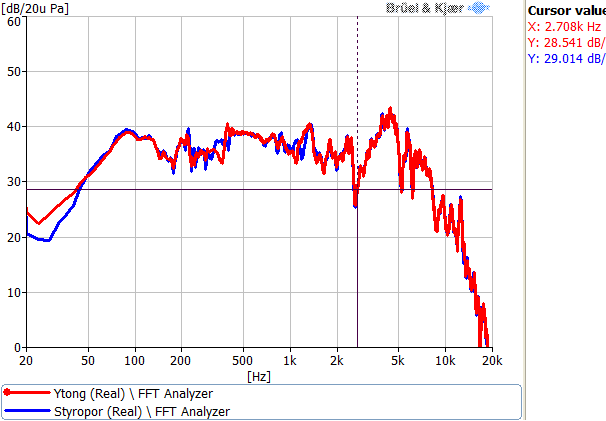
\includegraphics[width=0.75\textwidth]{img/Optimierung/Vergleich/VergleichYtognStyro_full.png}
	\caption{Vergleichsmessung Styropor zu Ytong-Ziegel von 20 Hz bis 20 kHz}
	\label{fig:4.4.1.1}
\end{figure}
\begin{figure} [H]
	\centering
	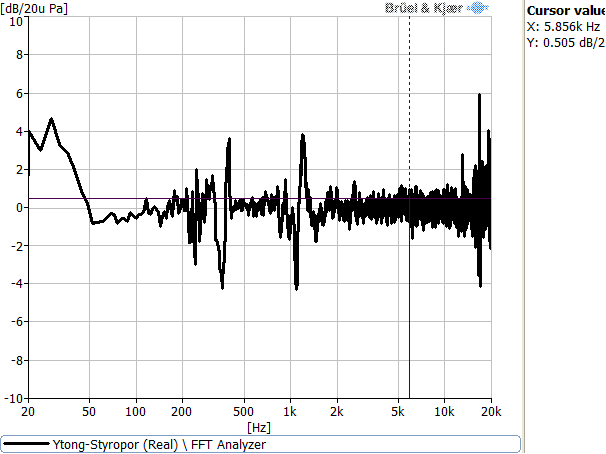
\includegraphics[width=0.75\textwidth]{img/Optimierung/Vergleich/VergleichYtognStyro_Abweichung_full.png}
	\caption{Vergleichsmessung Styropor zu Ytong-Ziegel von 20 Hz bis 20 kHz - Differenz der beiden Kurven}
	\label{fig:4.4.1.2}
\end{figure}


\begin{figure} [H]
	\centering
	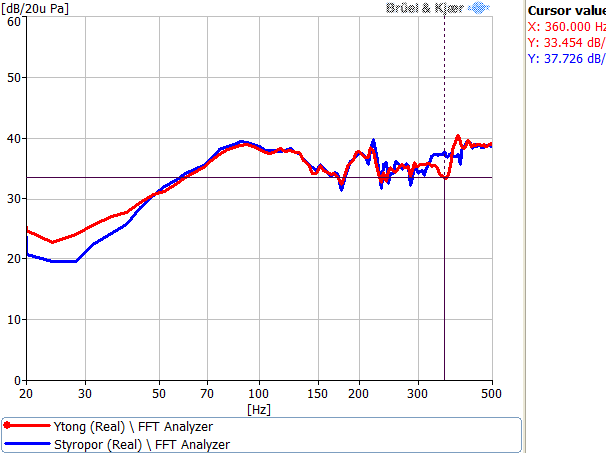
\includegraphics[width=0.75\textwidth]{img/Optimierung/Vergleich/VergleichYtognStyro_500Hz.png}
	\caption{Vergleichsmessung Styropor zu Ytong-Ziegel von 20 Hz bis 500 Hz}
	\label{fig:4.4.1.3}
\end{figure}
\begin{figure} [H]
	\centering
	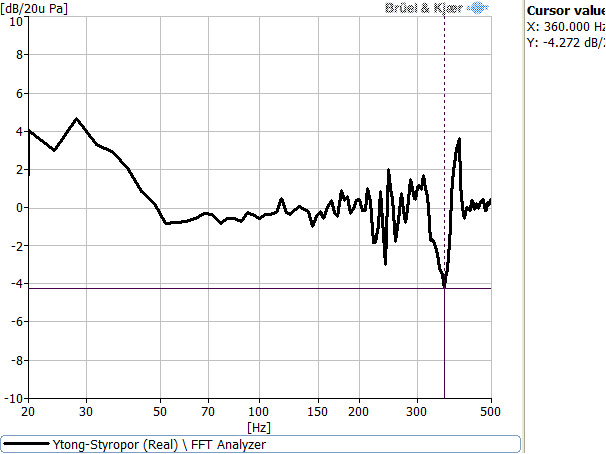
\includegraphics[width=0.69\textwidth]{img/Optimierung/Vergleich/VergleichYtognStyro_Abweichung_500Hz.png}
	\caption{Vergleichsmessung Styropor zu Ytong-Ziegel von 20 Hz bis 500 Hz - Differenz der beiden Kurven}
	\label{fig:4.4.1.4}
\end{figure}


\begin{figure} [H]
	\centering
	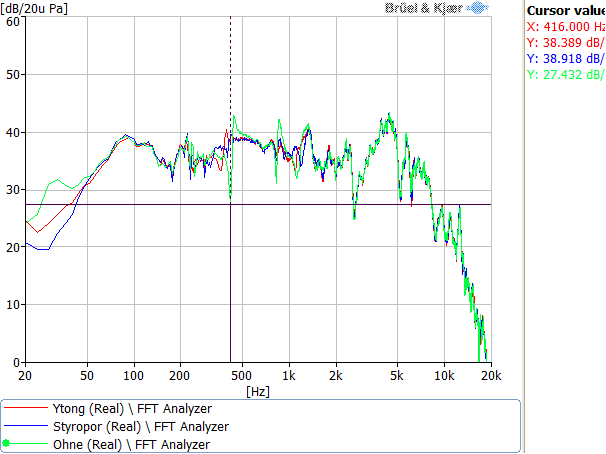
\includegraphics[width=0.69\textwidth]{img/Optimierung/Vergleich/VergleichYtognStyroOhne_full.png}
	\caption{Vergleichsmessung Styropor zu Ytong-Ziegel zu ohne Verminderung, von 20 Hz bis 20 kHz}
	\label{fig:4.4.1.5}
\end{figure}\begin{figure} [H]
	\centering
	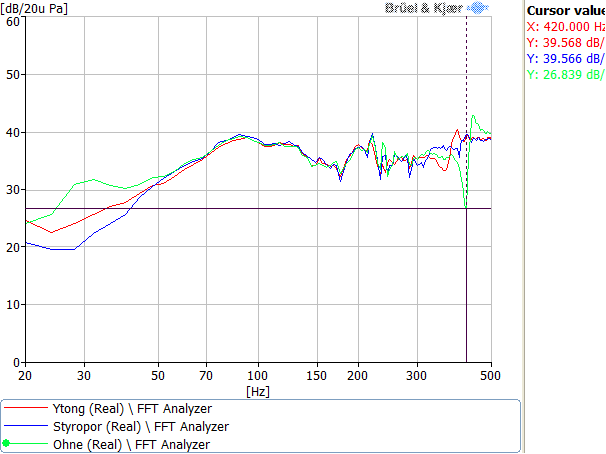
\includegraphics[width=0.7\textwidth]{img/Optimierung/Vergleich/VergleichYtognStyroOhne_500Hz.png}
	\caption{Vergleichsmessung Styropor zu Ytong-Ziegel zu ohne Verminderung, von 20 Hz bis 500 Hz}
	\label{fig:4.4.1.6}
\end{figure}

Die Schlussfolgerung aus diesen Messungen ist, dass Styropor sich auch zur Volumsverminderung von Lautsprechern gut eignet.
Aus diesem Grund wird Styropor auch hauptsächlich bei den folgenden Messungen verwendet.
%\\ \\

\newpage
\subsection{Subwoofer-Box}\label{subsec:4.4.2}
Das Ziel ist, die Box so klein wie möglich zu bauen, ohne Verlust an Klangqualität und Pegel.
Dafür wird die Messbox mit 149 l in ihrem Volumen vermindert, um zu testen, ob zuvor genannte Verluste auftreten.
Zu Beginn wird das Volumen drastisch verkleinert, in diesem Fall von 149 l auf 47,4 l (Bild \ref{fig:4.4.2.1}).

\begin{figure} [H]
	\centering
	\subfloat{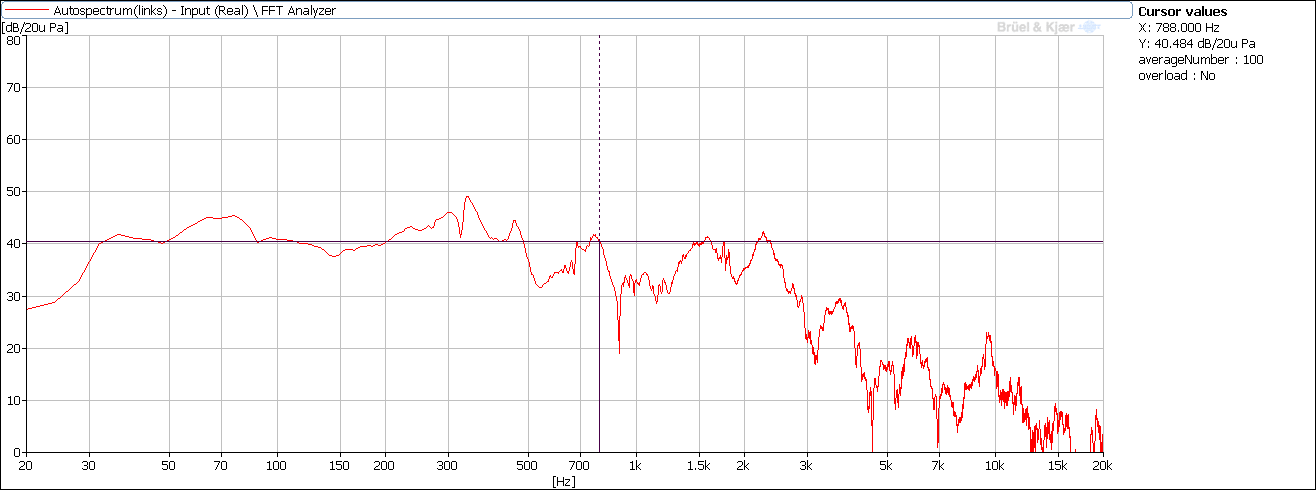
\includegraphics[width=1\textwidth]{img/LSMessung/TT/RenkforceOhneWolleMitSilikonV2.png}}\quad
	\subfloat{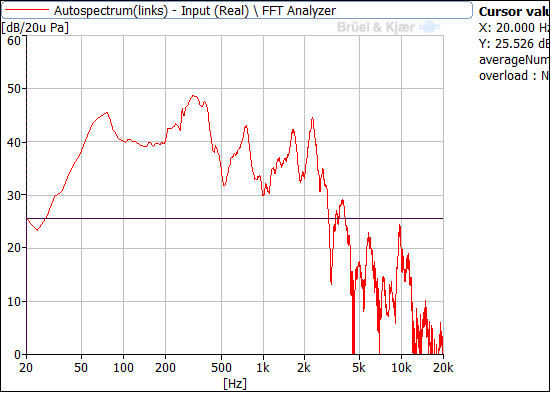
\includegraphics[width=0.65\textwidth]{img/Optimierung/Sub/RenkforceStyro_47l.png}}
	\caption{Renkforce Subwoofer: ohne Volumsverminderung (oben) - Boxenvolumen: 149 l | Mit Styropor (unten)\\- Boxenvolumen = 47,4 l}
	\label{fig:4.4.2.1}
\end{figure}

Leider wurde die Messung ohne Verringerung zu Beginn der Diplomarbeit dokumentiert, wo noch eine schlechtere Methode zur Dokumentation verwendet wurde.
Um die Kurven bewerten zu können, wurde, trotz falschen Formats, die Messung ohne Verringerung als Vergleich herangezogen.

\newpage
Die folgenden Messungen (ab nächster Seite) mit verschiedenen Volumina wurden an einem anderen Messtag erstellt.
In der Zwischenzeit wurden von anderen Personen ebenfalls Messungen erstellt, wobei das Verstärkerlevel des Messverstärkers verändert wurde.
Im ersten Moment wurde diese Änderung übersehen, jedoch nach Bemerken wieder an die einheitliche Messeinstellung angepasst.
Die vor Änderung aufgenommenen Kurven weisen einen um 8 dB höheren Pegel auf, als die danach aufgenommenen Kurven.
Um zu bestätigen, dass nicht die Volumsverminderung Schuld an der Pegeländerung ist, wurde eine Vergleichsmessung mit einem zuvor gemessenen Volumen angestellt.\\

\newpage
\textit{\textbf{ Die folgenden Messaufnahmen weisen einen um 8 dB erhöhten Pegel auf.}} Dazu gehören: Messung \ref{fig:4.4.2.2}, \ref{fig:4.4.2.3}, \ref{fig:4.4.2.4}, \ref{fig:4.4.2.5} und \ref{fig:4.4.2.6}\\

\begin{figure} [H]
\centering
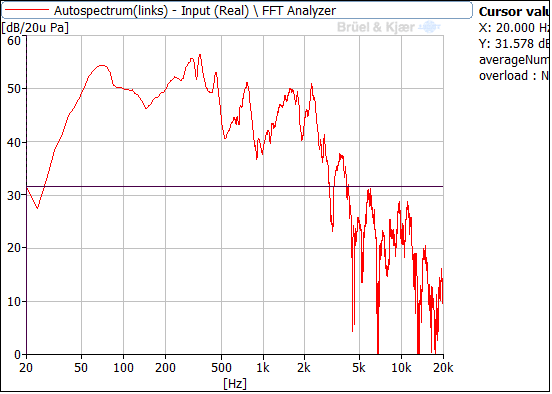
\includegraphics[width=0.74\textwidth]{img/Optimierung/Sub/RenkforceStyro_138l.png}
\caption{Renkforce Subwoofer: Styropor \\Volumen = 138,28 l}
\label{fig:4.4.2.2}
\end{figure}

\begin{figure} [H]
\centering
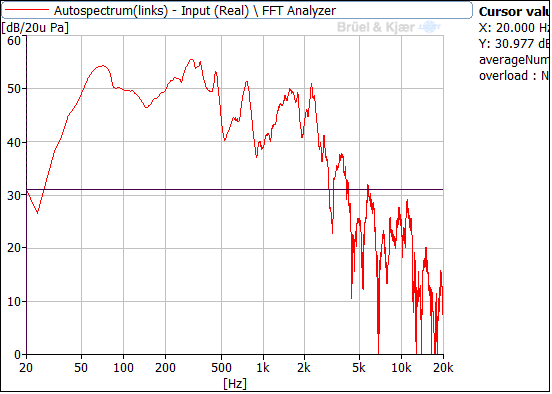
\includegraphics[width=0.74\textwidth]{img/Optimierung/Sub/RenkforceStyro_138l_Wolle.png}
\caption{Renkforce Subwoofer: Styropor, mit Polyesterwatte \\Volumen = 138,28 l}
\label{fig:4.4.2.3}
\end{figure}

\begin{figure} [H]
\centering
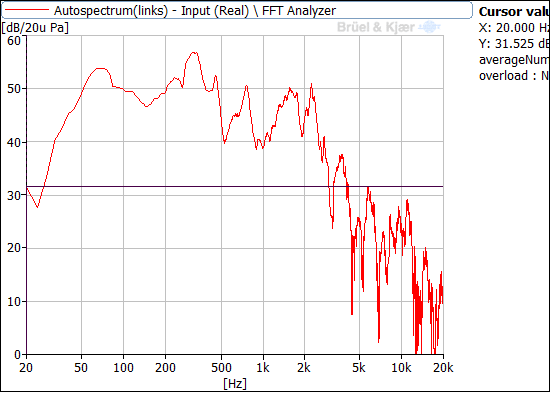
\includegraphics[width=0.75\textwidth]{img/Optimierung/Sub/RenkforceStyro_126l_Wolle.png}
\caption{Renkforce Subwoofer: Styropor, mit Polyesterwatte \\Volumen = 126,51 l}
\label{fig:4.4.2.4}
\end{figure}
\begin{figure} [H]
	\centering
	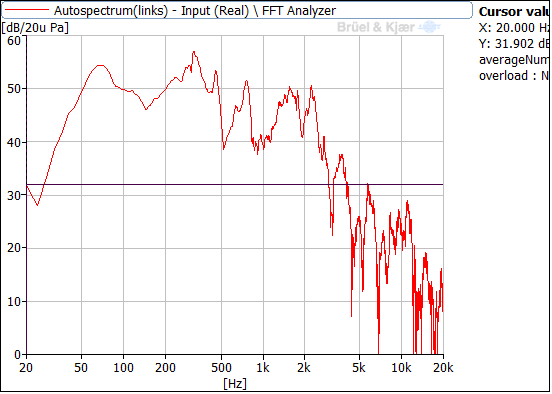
\includegraphics[width=0.75\textwidth]{img/Optimierung/Sub/RenkforceStyro_136l.png}
	\caption{Renkforce Subwoofer: Styropor \\Volumen = 136,84 l}
	\label{fig:4.4.2.5}
\end{figure}

\newpage
\textit{Die folgenden Messungen zeigen den Vergleich, von verstellter Ausgangsverstärkung zu einheitlichen verwendeten Ausgangsverstärkung. (Bild \ref{fig:4.4.2.6} und \ref{fig:4.4.2.7})}
\begin{figure} [H]
\centering
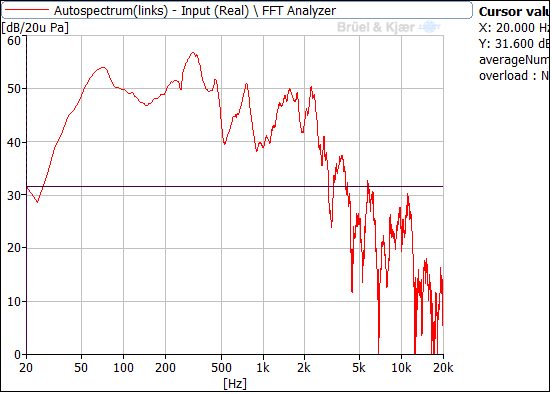
\includegraphics[width=0.65\textwidth]{img/Optimierung/Sub/RenkforceStyro_113l_Wolle.png}
\caption{Renkforce Subwoofer: Styropor und Ytong-Ziegel, mit Polyesterwatte \\Volumen = 113,25 l}
\label{fig:4.4.2.6}
\end{figure}

\begin{figure} [H]
\centering
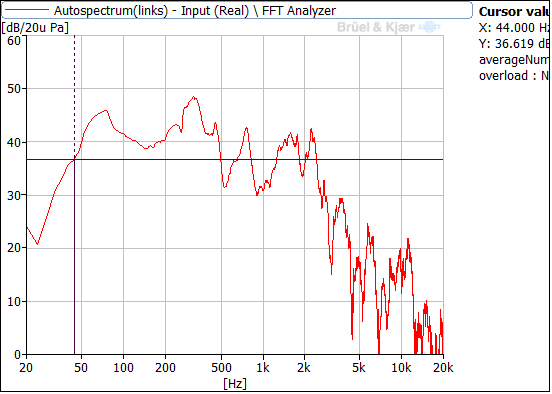
\includegraphics[width=0.65\textwidth]{img/Optimierung/Sub/RenkforceStyro_113l_Wolle_Angepasst.png}
\caption{Renkforce Subwoofer: Styropor und Ytong-Ziegel, mit Polyesterwatte - Angepasster Pegel \\Volumen = 113,25 l}
\label{fig:4.4.2.7}
\end{figure}
Beim Vergleich der beiden Kurven (Abb. \ref{fig:4.4.2.6} \& \ref{fig:4.4.2.7}) ist lediglich eine Verschiebung auf der Y-Achse merkbar.

\newpage
Nach den vielen verschiedenen Messungen, konnte der Schluss gezogen werden, dass ein Innenvolumen der Box von 47 Liter ausreicht, um die gleiche Klangqualität unter dem selben Schalldruckpegel zu erreichen.\\
Ein kleineres Volumen wurde nicht angestrebt, da die ganze Elektronik ( Verstärker, Weichen, Akku, ...) ebenfalls in der Box Platz haben soll.
Aus diesem Grund wird eine Box (Kap. \ref{sec:8.11}) mit einem Innenvolumen von 72 Litern angestrebt.\\ \\ \\ \\




\subsection{Box für Satelliten-Boxen}\label{subsec:4.4.3}
Gleich wie für die Subwoofer-Box gilt auch hier das Boxenvolumen weitestgehend zu vermindern, unter der Bedingung, dass Klangqualität und Schalldruckpegel nicht darunter leiden.
Hier wird die Tiefton-Lautsprecher-Box mit 13,72 l als Messbox verwendet.
Mit verschiedenen Volumina und mit oder ohne Polyesterwatte wird das Tiefton-Lautsprecher-Chassis \enquote{TT1} gemessen.\\
Zuallererst wird der Extremvergleich angestellt.
Die Messung \ref{fig:4.4.3.1} wurde ohne Styropor und ohne Polyesterwatte aufgenommen.
Im Vergleich zu dieser steht die Messung \ref{fig:4.4.3.2}.
Diese wurde mit einem durch Styropor verringerten Volumen gemessen, sodass die Box ein Innenvolumen von 4,87 l hatte.

\newpage
\begin{figure} [H]
	\centering
	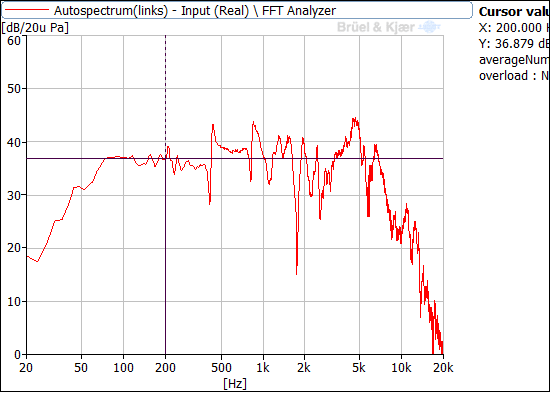
\includegraphics[width=0.75\textwidth]{img/Optimierung/TT/TT1_ohneAllem.png}
	\caption{PSS 297 58206 (\enquote{TT1}) ohne Volumsverminderung \\Volumen = 13,72 l}
	\label{fig:4.4.3.1}
\end{figure}

\begin{figure} [H]
	\centering
	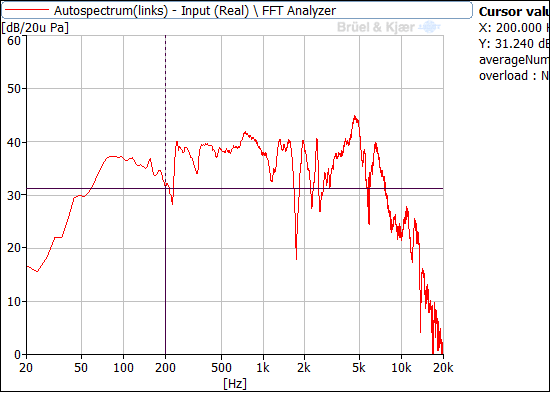
\includegraphics[width=0.75\textwidth]{img/Optimierung/TT/TT1_Styro_4-87l.png}
	\caption{PSS 297 58206 (\enquote{TT1}) Volumsverminderung durch Styropor \\Volumen = 4,87 l}
	\label{fig:4.4.3.2}
\end{figure}

%TD Bitte Korregieren falls ich mich vertan habe!
\newpage
Als nächstes wurde versucht, den Einbruch in der Frequenzgangskurve bei 1.75 kHz zu verhindern.
Ein möglicher Grund für diesen Einbruch kann eine Resonanz in der Box aufgrund der Seitenwandlänge sein.
Diese Annahme kommt daher, dass die Seitenlänge der Box relativ lang ist und möglicherweise genau $\frac{\lambda}{2}$ für den verwendeten Frequenzbereich bedeutet und dadurch die an der Rückwand reflektierte Welle mit der hinlaufenden Welle interferiert.
Es entsteht eine Resonanz mit der Box.
Es wird deshalb eine Schraubzwinge mittig der Seitenwand auf der Box montiert, um die mögliche Resonanz zu unterbinden.
%WAtch here please!
%Durch das anbringen der Schraubzwinge wird die Seitenwand in der Mitte stabiler, teilt daher die Seitenlänge in der Mitte und verhindert so das Mitschwingen der Wand für die Frequenz resultierend aus der Länge.
Als Vergleich wird die Messung mit selbigen Volumsbedingungen und ohne Schraubzwinge herangezogen (Bild \ref{fig:4.4.3.1}).
Die Messung mit Schraubzwinge ergibt aber keinen wesentlichen Unterschied (Bild \ref{fig:4.4.3.3}).\\ \\

\begin{figure} [H]
	\centering
	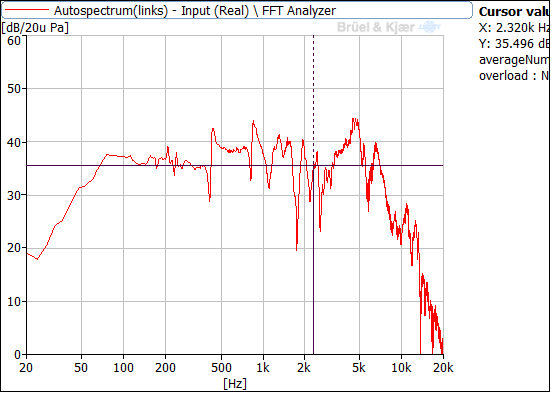
\includegraphics[width=0.75\textwidth]{img/Optimierung/TT/TT1_ohneAllem_Schraubzwinge.png}
	\caption{PSS 297 58206 (\enquote{TT1}) ohne Volumsverminderung, mit Schraubzwinge \\Volumen = 13,72 l}
	\label{fig:4.4.3.3}
\end{figure}

\newpage
Nachfolgend wurden weitere Kurven unter Volumsänderung aufgenommen.

\begin{figure} [H]
	\centering
	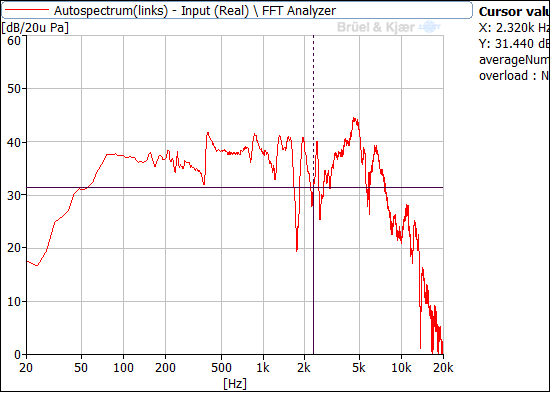
\includegraphics[width=0.75\textwidth]{img/Optimierung/TT/TT1_Styro_9-67l.png}
	\caption{PSS 297 58206 (\enquote{TT1}) ohne Volumsverminderung \\Volumen = 9,67 l}
	\label{fig:4.4.3.4}
\end{figure}

\begin{figure} [H]
	\centering
	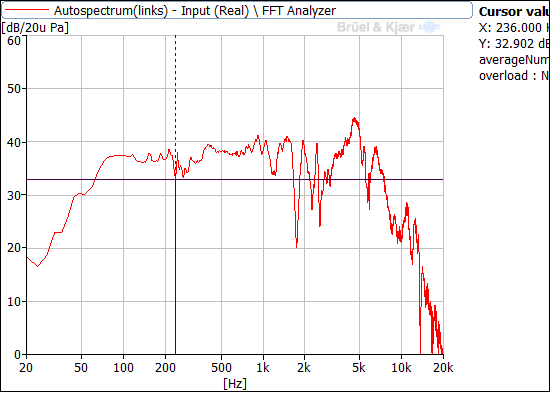
\includegraphics[width=0.75\textwidth]{img/Optimierung/TT/TT1_Styro_7-17l.png}
	\caption{PSS 297 58206 (\enquote{TT1}) ohne Volumsverminderung \\Volumen = 7,17 l}
	\label{fig:4.4.3.5}
\end{figure}

\begin{figure} [H]
	\centering
	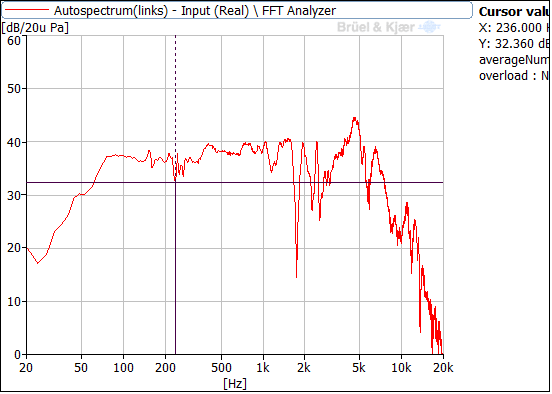
\includegraphics[width=0.7\textwidth]{img/Optimierung/TT/TT1_Styro_6-07l.png}
	\caption{PSS 297 58206 (\enquote{TT1}) ohne Volumsverminderung \\Volumen = 6,07 l}
	\label{fig:4.4.3.6}
\end{figure}

\begin{figure} [H]
	\centering
	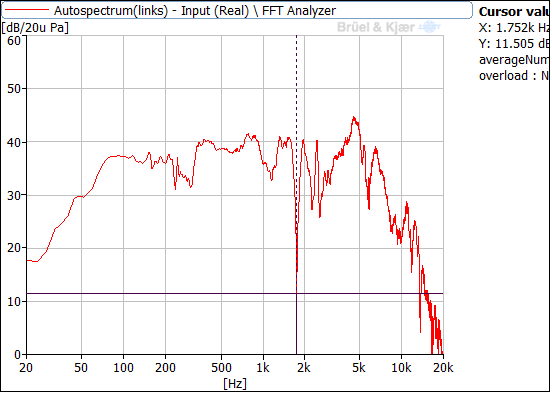
\includegraphics[width=0.7\textwidth]{img/Optimierung/TT/TT1_Styro_5-47l.png}
	\caption{PSS 297 58206 (\enquote{TT1}) ohne Volumsverminderung \\Volumen = 5,47 l}
	\label{fig:4.4.3.7}
\end{figure}

\textbf{Schlussendlich erschien die Messkurve \ref{fig:4.4.3.5} als beste Kurve, da sie in einem Bereich von ungefähr 60 Hz bis 1,7 kHz eine geringe Welligkeit aufweist (> +/- 5 dB).
Aus diesem Grund wird ein Satelliten-Boxen-Volumen von 7 Liter angestrebt.}

